\section{Miary ewaluacji}
W celu oceny skuteczności systemu detekcji wykorzystano następujących miary:
\begin{itemize}
    % \item pole powierzchni pod krzywą Receiver Operating Characteristic (ROC)
    \item  precyzja dla top n obserwacji (P@N)
    \item pole powierzchni pod krzywą Receiver Operating Characteristic (ROC)

\end{itemize}
Wykorzystane metryki wybrane były jako informatywny sposób oceny skuteczności detekcji anomalii \cite{campos2016evaluation}. Jak również wykorzystane były w benchmarku algorytmów zawartego w dokumentacji biblioteki PyOD.

\subsection{Precyzja dla top n obserwacji (P@N)}
    Miara oblicza precyzję dla top n obserwacji, gdzie n oznaczać będzie sumę obserwacji odstających w zbiorze danych. N obserwacji, którym system nadał najwyższą wartość wskaźnika anomalności, zaklasyfikowane zostały jako anomalie. P@N określa stosunek klasyfikacji prawdziwie pozytywnych (TP) do sumy klasyfikacji prawdziwie pozytywnych (TP) i fałszywie pozytywnych (FP) dla N obserwacji zaklasyfikowanych jako anomalie:
    \begin{equation}
        P@N = \frac{TP}{TP+FP}
    \end{equation}
\subsection{Pole powierzchni pod krzywą Receiver Operating Characteristic (ROC)}
    Miara określa prawdopodobieństwo, że losowy element klasy pozytywnej(anomalii) otrzyma wyższą wartość anomalności niż losowo wybrany element klasy negatywnej (poprawna obserwacja). Krzywa ROC:
    \begin{figure}[!h]
        \centering
        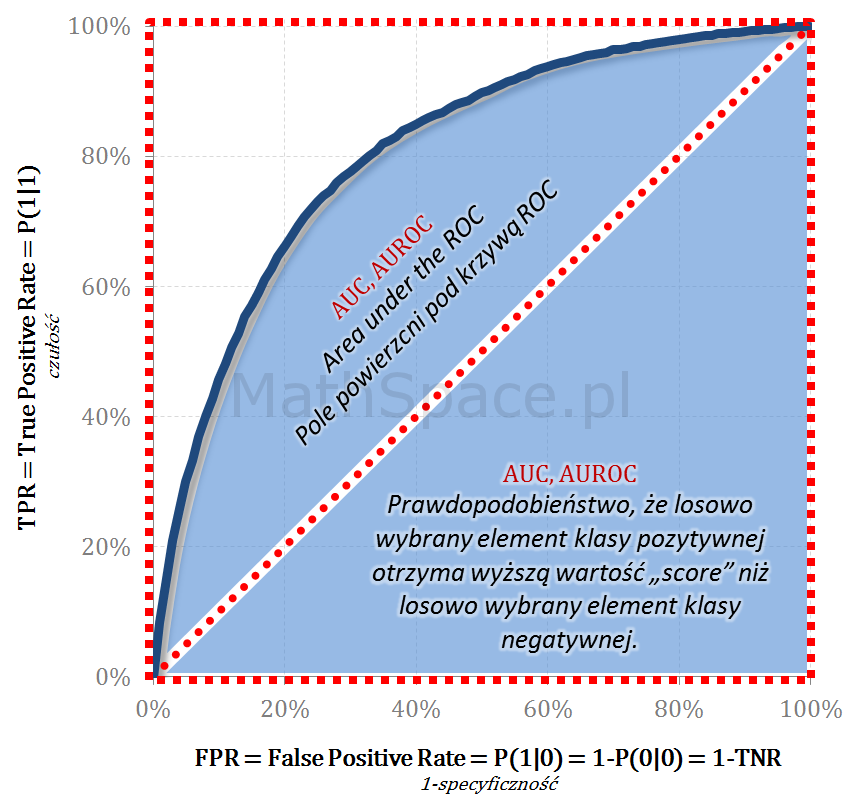
\includegraphics[width = 0.6\textwidth]{chapters/analiza/img/ROC-interpr-AUROC.png}
        \caption{Interpretacja pola pod krzywą ROC}
        \footnotesize{źródło: \cite{roc-image} }
        \label{fig:my_label}
    \end{figure}
% \begin{itemize}
%     \item pole powierzchni pod krzywą Receiver Operating Characteristic (ROC) \\
%     miara określa prawdopodobieństwo, że losowy element klasy pozytywnej(anomalii) otrzyma wyższą wartość anomalności niż losowo wybrany element klasy negatywnej (poprawna obserwacja). Krzywa ROC:
%     \begin{figure}[!h]
%         \centering
%         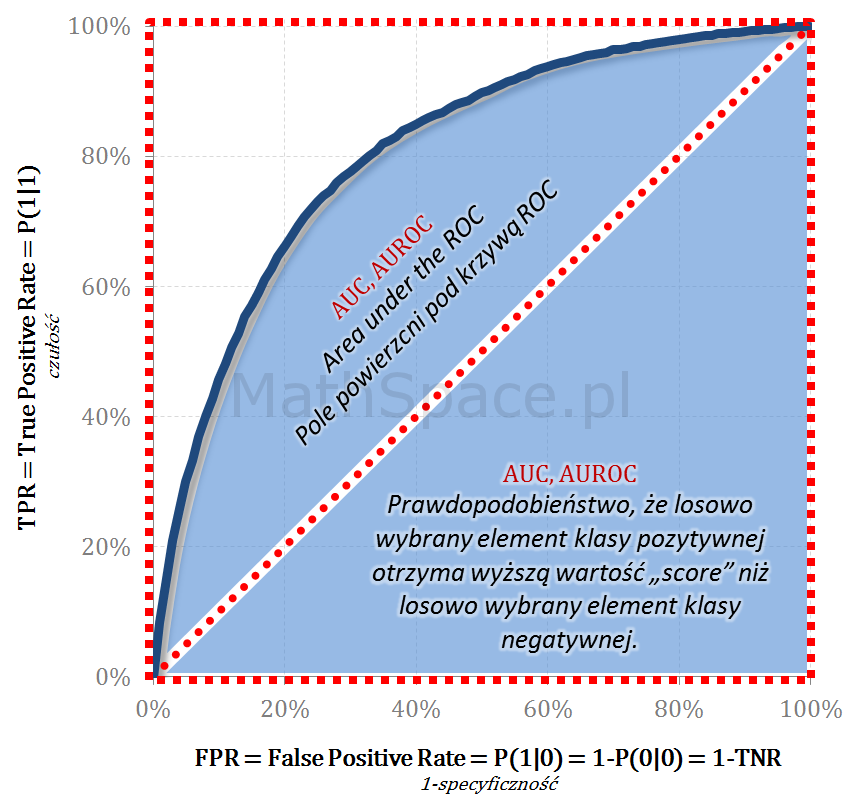
\includegraphics[width = 0.6\textwidth]{chapters/analiza/img/ROC-interpr-AUROC.png}
%         \caption{Interpretacja pola pod krzywą ROC}
%         \footnotesize{źródło: \cite{roc-image} }
%         \label{fig:my_label}
%     \end{figure}
%     \item precyzja dla top n obserwacji (P@N) \\
%     miara oblicza precyzję dla top n obserwacji, gdzie n oznaczać będzie sumę obserwacji odstających w zbiorze danych. N obserwacji, którym system nadał najwyższą wartość wskaźnika anomalności, zaklasyfikowane są jako anomalie. Precyzja określa stosunek klasyfikacji prawdziwie pozytywnych (TP) do sumy klasyfikacji prawdziwie pozytywnych (TP) i fałszywie pozytywnych (FP):
%     \begin{equation}
%         precyzja = \frac{TP}{TP+FP}
%     \end{equation}
% \end{itemize}
% Wykorzystane metryki wybrane były jako informatywny sposób oceny skuteczności detekcji anomalii \cite{campos2016evaluation}. Jak również wykorzystane były w benchmarku algorytmów zawartego w dokumentacji biblioteki PyOD.

\section{Wykorzystane zbiory danych }
Wykorzystano bazę zbiorów danych ODDS \cite{ODDS}. W celu ewaluacji wykorzystano zbiory danych, dla których w dokumentacji biblioteki PyOD przeprowadzono analizę skuteczności detekcji anomalii dla wybranych zbiorów danych.
% \begin{sidewaystable}
%     \centering
\begin{table}[h]
    \centering
\begin{tabularx}{\textwidth}{lXX}
\toprule
      Zbiór & Charakter zbioru danych  &  Znaczenie anomalii  \\ \hline
\midrule
arrhythmia &     Dane pacjenta wraz z informacjami badania EKG & Wykrycie arytmi serca \\
    cardio &    Wyniki badania Kardiotokografii   &  Wykrycie patologii pracy serca płodu      \\
     glass &       Skład chemiczny różnych rodzai szkła  & Wykrycie próbek szkła, należących do klasy zdecydowanie mniejszościowej  \\
ionosphere & Sygnały odbite radaru (jonosondy)  &  Sygnał jonosondy przechodzi przez jonosferę -- brak wykrycia struktury w jonosferze    \\   
    letter & Wybrane 3 litery tworzą klasę normalnych obserwacji &  Litery spoza normalnej klasy  \\    
    lympho &  Wyniki badania limfografii  &  Wykrycie metastazy lub zwłóknienia   \\
     mnist &  Obserwacje cyfry 0 uznane za normalne obserwacje  & 700 zdjęć cyfry 6 uznane za anomalie  \\
      musk & Zbiór opisuje budowę oraz strukturę różnych związków chemicznych & Wykrycie związku uznanego za piżmo \\
 optdigits &  Zbiór składa się z cyfr. Zbiór zawiera ponad 97\% obserwacji cyfr od 1 do 9 &            Wykrycie cyfry 0 (2.86\%) -- anomalia \\
 pendigits & Zbiór zbliżony charakterem do ,,optdigits'' &  Wykrycie cyfry 0 -- anomalia     \\
      pima & Zbiór danych o kobietach z plemienia Pima takich jak poziom glukozy, BMI, ciśnienie tętnicze &      Wykrycie cukrzycy        \\
 satellite & Zdjęcia satelitarne programu Landsat. Zbiór danych oryginalnie służył do klasyfikacji gleby (7 klas)   &   Najmniej liczne klasy (2,4,5) -- anomalie      \\
satimage-2 &  Zbiór danych ,,satellite'' dla którego ilość obserwacji klasy 2 została zmniejszona do 71 &   Wykrycie gleby należącej do klasy 2 (pole bawełny)       \\
   shuttle & Informacje pokładowe wahadłowca kosmicznego. Ponad 92\% obserwacji należy do klasy 1 &    Obserwacje nie należące do klasy 1 -- anomalie        \\
 vertebral &  Cechy biometryczne opisujące miednicę oraz odcinek lędzwiowy kręgosłupa   &            Obserwacje normalnej biomechaniki zmniejszono do 30 obserwacji -- anomalie  \\
    vowels & Dane zawierają zakodowane wypowiedzenia samogłoski {/ae/}, przez 4 mężczyzn. Wypowiedzenia samogłoski przez pierwszego mężczyzny zmniejszono do 50 & Wykrycie wypowiedzenia samogłoski /ae/ przez 1 mężczyznę  -- anomalia         \\
       wbc &   Wyniki biopsji aspiracyjnej cienko-igłowej guzów piersi & Żłośliwy rak piersi -- anomalia.
\bottomrule
\end{tabularx}
    \caption{Informacje o charakterze zbioru danych i obecnych w zbiorze anomalii}
    \footnotesize{źródło: Opracowanie własne na podstawie \cite{ODDS}}
    \label{tab:my_label}
\end{table}
% \end{sidewaystable}
% \begin{sidewaystable}
%     \centering
\begin{table}[h]
    \centering
\begin{tabularx}{\textwidth}{lXXXXXXX}
\toprule
      Zbiór &  Liczba Obserwacji &   Liczba Cech &  Procent Anomalii &  Brakujące wartości & Cechy jakościowe & Cechy ilościowe \\ \hline
\midrule
arrhythmia &       452 &           274 &       14.6018 & Tak & Tak & Tak \\
    cardio &      1831 &            21 &        9.6122 & Nie & Nie & Tak  \\
     glass &       214 &             9 &        4.2056 & Nie & Nie & Tak \\
ionosphere &       351 &            33 &       35.8974 & Nie & Nie & Tak \\
    letter &      1600 &            32 &        6.2500 & Nie & Nie & Tak \\
    lympho &       148 &            18 &        4.0541 & Nie & Tak & Nie \\
     mnist &      7603 &           100 &        9.2069 & Nie & Nie & Tak \\
      musk &      3062 &           166 &        3.1679 & Nie & Nie & Tak \\
 optdigits &      5216 &            64 &        2.8758 & Nie & Nie & Tak \\
 pendigits &      6870 &            16 &        2.2707 & Nie & Nie & Tak \\
      pima &       768 &             8 &       34.8958 & Nie & Nie & Tak \\
 satellite &      6435 &            36 &       31.6395 & Nie & Nie & Tak \\
satimage-2 &      5803 &            36 &        1.2235 & Nie & Nie & Tak \\
   shuttle &     49097 &             9 &        7.1511 & Nie & Nie & Tak \\
 vertebral &       240 &             6 &       12.5000 & Nie & Nie & Tak \\
    vowels &      1456 &            12 &        3.4341 & Nie & Nie & Tak \\
       wbc &       378 &            30 &        5.5556 & Nie & Nie & Nie \\
\bottomrule
\end{tabularx}
    \caption{Informacje o właściwościach zbiorów danych}
    \footnotesize{źródło: Opracowanie własne na podstawie \cite{ODDS}}
    \label{tab:my_label}
\end{table}
% \end{sidewaystable}